\RequirePackage{atbegshi}
\documentclass{beamer}

%\usepackage{beamerarticle}

\usepackage{beamerthemesplit}
\usepackage{graphicx}
\usepackage{xypic}
\usepackage{wrapfig}

\title{A Radio Relay System for Remote Sensors in the Antarctic (or anywhere!)}
\subtitle{Final Seminar}
\author{Mark Jessop}
\date{September 27, 2010}



\begin{document}

\frame{
\titlepage
\begin{center}
\small{Supervisor: Dr Chris Coleman}% \hspace{20pt} Co-Supervisor: Dr  Said Al-Sarawi}
\end{center}
}

%\section[Outline]{}
%\frame{\tableofcontents}

\section{Introduction}

\subsection{Project Aim}
\frame{
\frametitle{Project Aim}
\begin{itemize}
\item Design and build a low power HF data transmitter for use in remote sensor systems.
\item Originally intended for use in the Antarctic.
\item Can be used anywhere!
\end{itemize}
}

\subsection{Hardware \& Software Overview}
\frame{
\frametitle{Hardware \& Software Overview}
\begin{itemize}
\item Atmel XMega Micro-controller
\item Analog Devices AD9835 Signal Generator IC
\item Class E Power Amplifier
\end{itemize}
}

\section{Hardware}

\subsection{CPU}
\frame{
\frametitle{CPU - Atmel ATXmega128A1}
\begin{figure}
  \begin{center}
    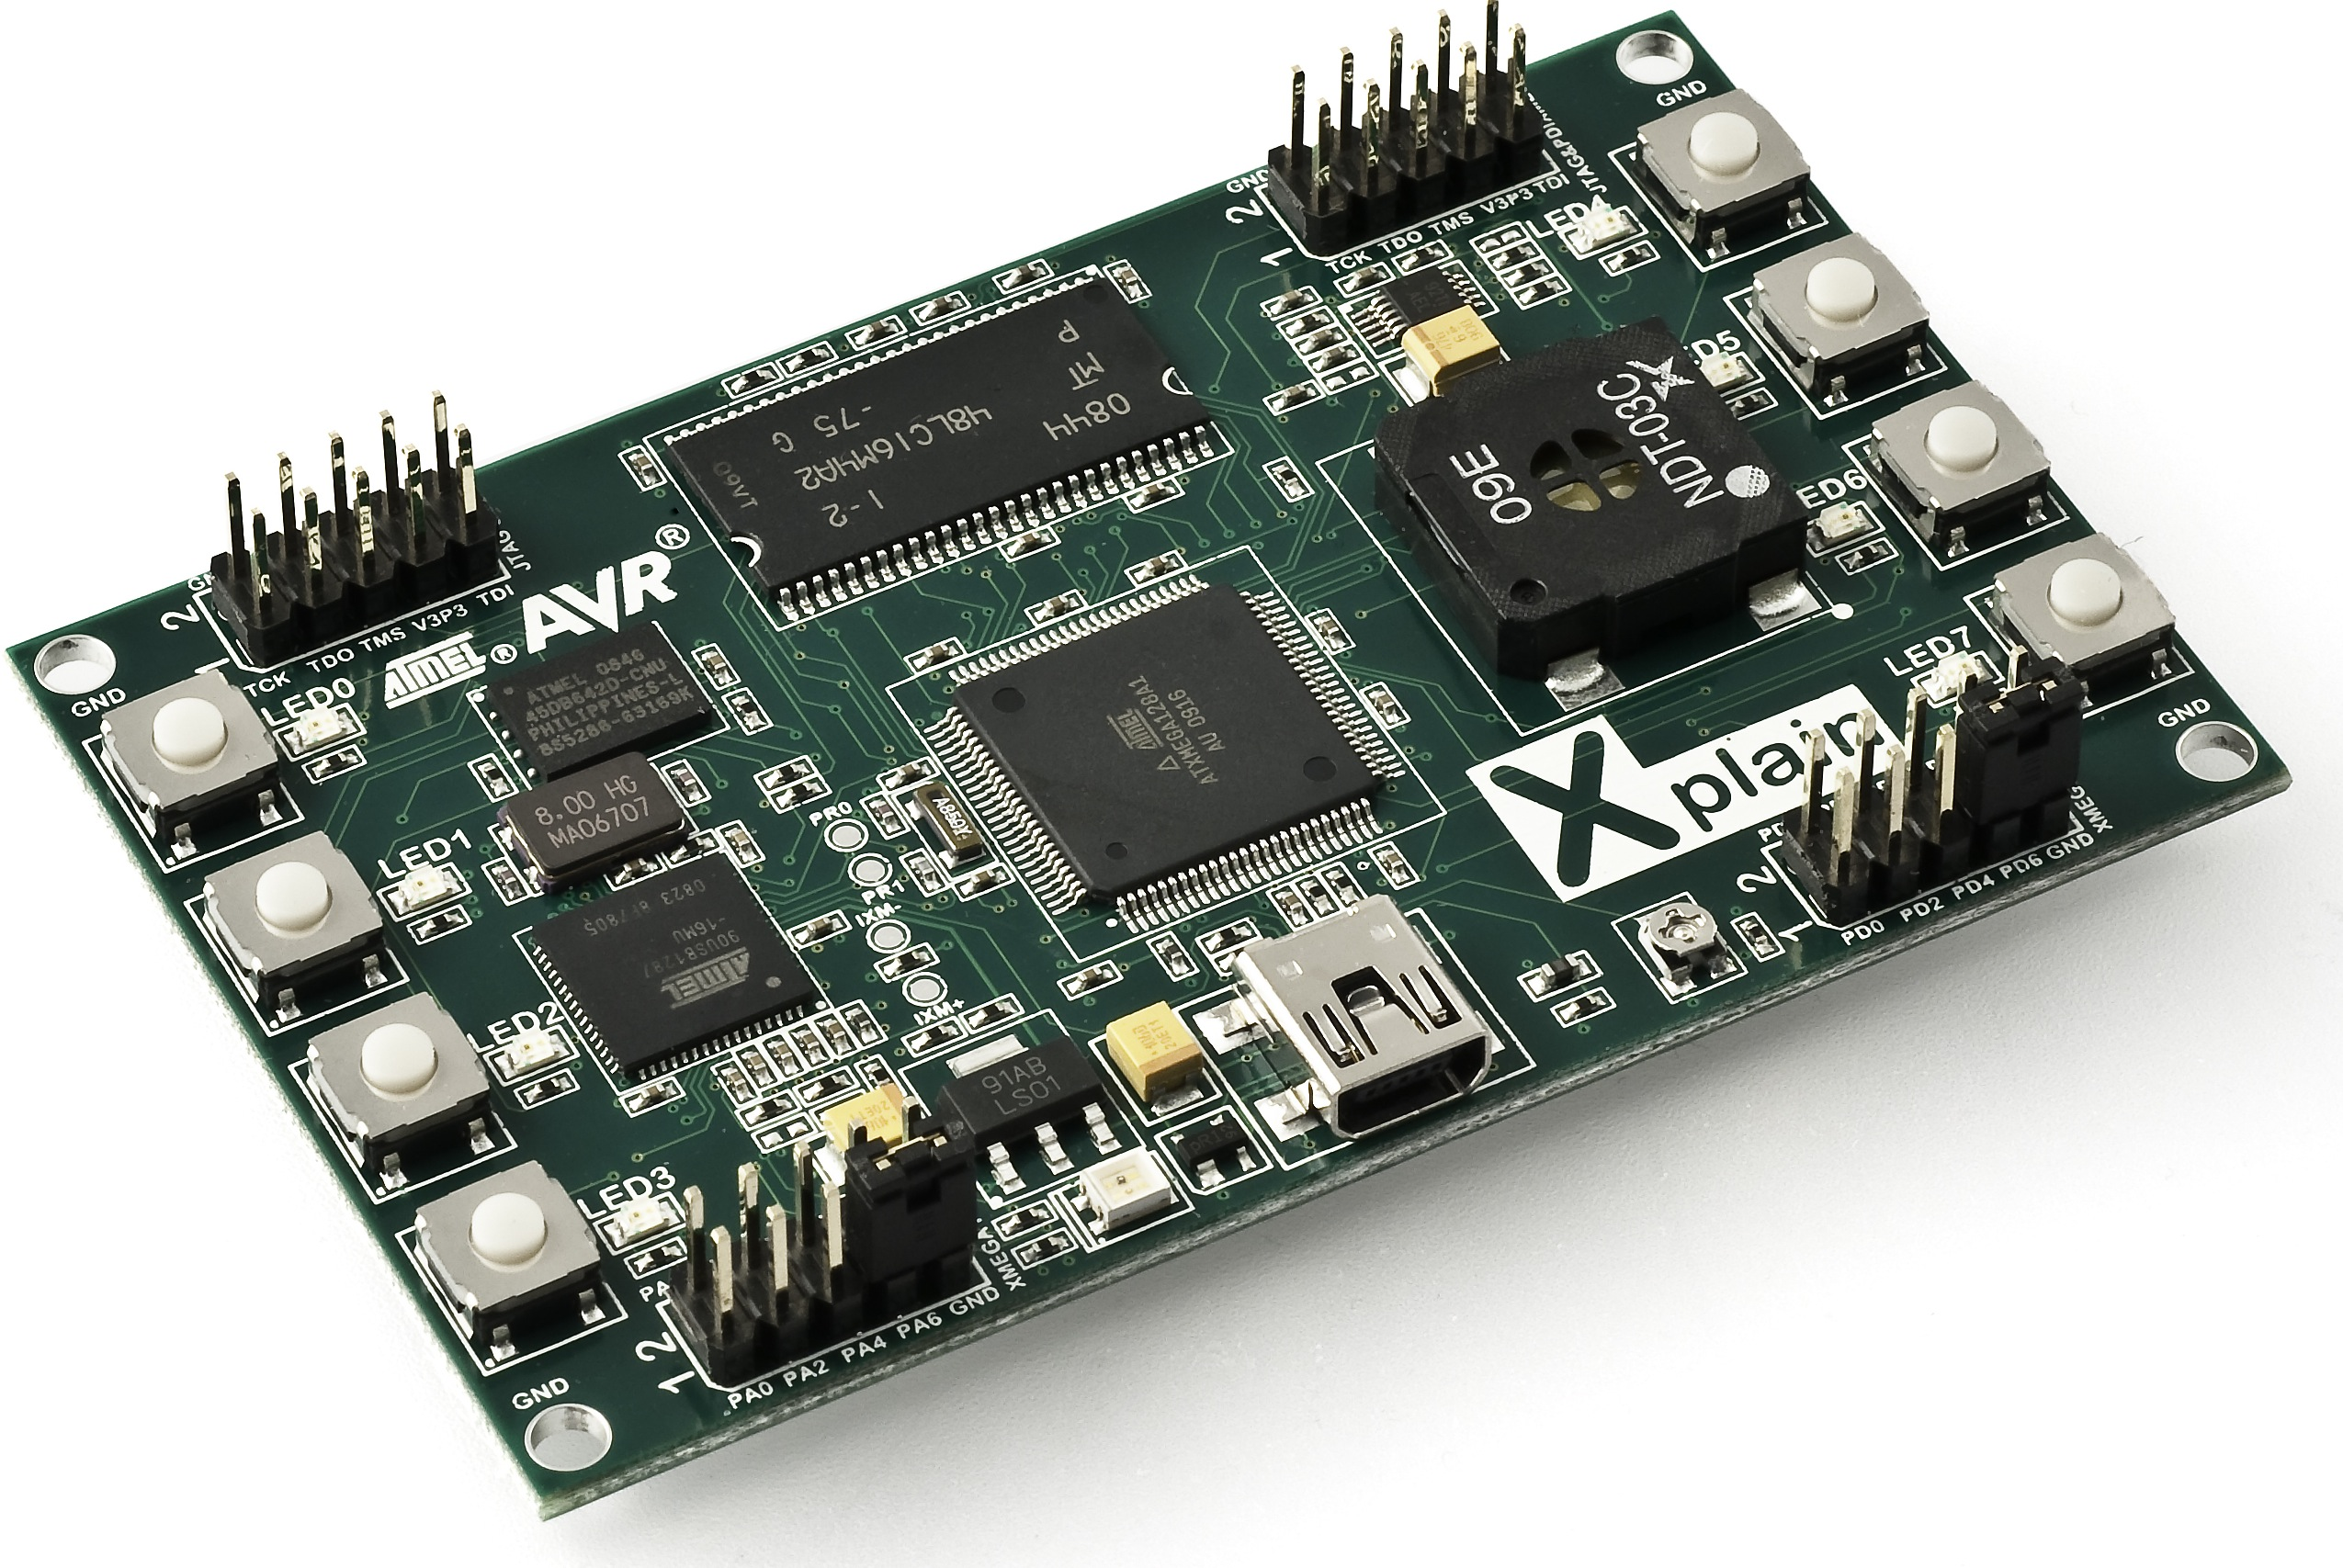
\includegraphics[width=0.5\textwidth]{images/xplain.jpg}
  \end{center}
  %\caption{Atmel XPlain Development Board}
  \label{xplain}
\end{figure}
\textbf{Atmel XPlain Development Board}
\begin{itemize}
\item Atmel ATXmega128A1 Micro-Controller, clocked at 32MHz
\item 8MB SDRAM
\item 8MB NAND Flash Memory
\item Low Power Consumption - 18mA @ 32MHz, 1.4mA @ 2MHz, $1.16\mu A$ Power-Save
\end{itemize}
}

\subsection{Signal Generator}
\frame{
\frametitle{Signal Generator - Analog Devices AD9835}
\begin{itemize}
\item Original intention was to use an AD9834
\item AD9835 Board ended up having the same power requirements!
\end{itemize}

\begin{figure}
  \begin{center}
    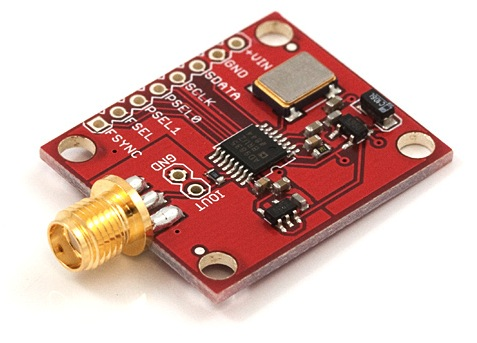
\includegraphics[width=0.25\textwidth]{images/ad9835.jpg}
  \end{center}
  %\caption{Atmel XPlain Development Board}
  \label{ad9835}
\end{figure}
\textbf{Analog Devices AD9835}
\begin{itemize}
\item Can generate Sine-waves between 1Hz - 25MHz.
\item 2 programmable (via SPI) frequency registers.
\item Dedicated pins for switching between registers.
\item Using 16MHz SPI clock, can reprogram at 7500Hz.
\end{itemize}



}

\end{document}